\section{Rank measures against noise}
\label{sec:results}

\subsection{Three of four measures barely separate an update from noise}
\label{sec:metrics}

\begin{figure}[t]
\begin{center}
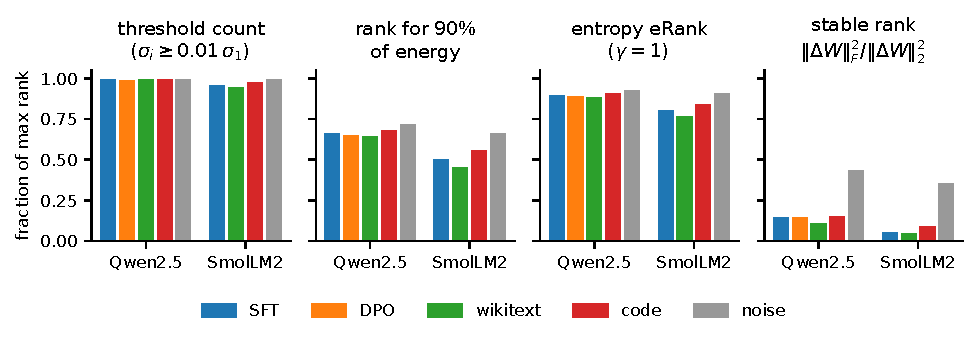
\includegraphics[width=\linewidth]{figures/metrics_vs_noise.pdf}
\end{center}
\caption{Four rank measures for our fine-tuning updates and for the random-init
pair of the same architecture (grey). The threshold count, the 90\%-energy rank
and the entropy effective rank put every update close to the noise value;
stable rank puts every update far below it. Means over 168 (Qwen2.5-0.5B) and
224 (SmolLM2-360M) matrices; DPO is measured against the SFT checkpoint.}
\label{fig:metrics}
\end{figure}

\begin{table}[t]
\caption{Rank measures as a fraction of the maximum rank, and the share of
energy in the top singular value. Last column: how many times lower the
update's stable rank is than the noise baseline's, with 95\% layer-bootstrap
intervals.}
\label{tab:metrics}
\begin{center}
\small
\begin{tabular}{llcccccc}
\toprule
 & & threshold & 90\% energy & eRank & stable & top-1 & noise / real \\
model & update & $\thresholdrank$ & $\energyrank$ & $\gamma=1$ & $\stablerank$ & energy & (stable) \\
\midrule
Qwen2.5-0.5B & SFT              & 0.991 & 0.660 & 0.893 & 0.145 & 5.1\% & 3.0 (2.7--3.4) \\
             & DPO (vs SFT)     & 0.990 & 0.652 & 0.891 & 0.144 & 5.5\% & 3.0 (2.7--3.4) \\
             & wikitext LM      & 0.990 & 0.643 & 0.881 & 0.110 & 6.9\% & 3.9 (3.5--4.5) \\
             & code LM          & 0.992 & 0.679 & 0.905 & 0.154 & 3.0\% & 2.8 (2.6--3.1) \\
             & random-init pair & 0.996 & 0.716 & 0.928 & 0.436 & 0.6\% & -- \\
\midrule
SmolLM2-360M & SFT              & 0.955 & 0.500 & 0.800 & 0.052 & 7.8\% & 6.9 (6.2--7.7) \\
             & wikitext LM      & 0.943 & 0.452 & 0.767 & 0.045 & 9.2\% & 7.9 (7.3--8.7) \\
             & code LM          & 0.976 & 0.559 & 0.841 & 0.089 & 4.7\% & 4.0 (3.6--4.5) \\
             & random-init pair & 0.996 & 0.659 & 0.908 & 0.354 & 0.5\% & -- \\
\bottomrule
\end{tabular}
\end{center}
\end{table}

Figure~\ref{fig:metrics} and Table~\ref{tab:metrics} compare the four measures
on our updates. The threshold count puts the Qwen updates at 99.0--99.2\% of
full rank against 99.6\% for the random-init pair, and the SmolLM2 updates at
94--98\% against 99.6\%. Read on its own, this says fine-tuning produces
updates of essentially full rank, which is how we first read it.
The 90\%-energy rank and the entropy effective rank move in the right
direction but by little: 0.64--0.68 against 0.72, and 0.88--0.91 against 0.93,
on Qwen. Stable rank instead puts every update 2.8--7.9$\times$ below the noise
baseline, with intervals far from 1.

The gap is consistent rather than random: the layer-bootstrap interval on the
noise-to-real ratio of the entropy effective rank stays above 1 for every run
(the closest is the code control, 1.023--1.030). So eRank does register the
structure, compressed into a few percent, where stable rank shows it as a
several-fold difference. Weighting $\sigma_i$ linearly inside an entropy lets
the long, flat part of the spectrum dominate.

The effect holds for every matrix type. For the Qwen SFT update, stable rank
is lower than noise by 3.7$\times$ for \texttt{q\_proj}, 5.1$\times$ for
\texttt{up\_proj} and 1.7$\times$ for \texttt{v\_proj}, the weakest case
(Appendix~\ref{app:pertype}).

\subsection{A noise-like tail and a few dominant directions}
\label{sec:headtail}

The measures disagree because the updates have two parts. The top of the
spectrum is far more concentrated than noise: the top singular value of the
Qwen SFT update holds 5.1\% of its energy against 0.6\% for the random pair,
the top 8 hold 12.0\% against 4.9\%, and the top 32 hold 26.0\% against
17.5\%. Below that, the spectrum decays slowly, much like a random matrix's.
Stable rank is dominated by the top, so it sees the concentration. The
threshold count and the energy rank count directions, most of which sit in
the tail, so they see a high-rank matrix. The entropy effective rank sits in
between.

Both statements, ``fine-tuning updates are high rank'' \citep{biderman2024lora}
and ``fine-tuning updates are concentrated'', are therefore true of the same
matrices. Which one a paper reports depends on the measure, and without a
noise baseline neither number says how much structure there is. The tail is
not negligible either: \S\ref{sec:cutoff} shows that deleting it hurts.

\subsection{Concentration is a property of fine-tuning, not of alignment}
\label{sec:controls}

\begin{table}[t]
\caption{Paired differences in stable rank (fraction of maximum rank) between
runs on the same base model, with 95\% layer-bootstrap intervals. Seed
differences compare runs with a different training seed and data sample.}
\label{tab:paired}
\begin{center}
\begin{tabular}{lcc}
\toprule
paired difference & Qwen2.5-0.5B & SmolLM2-360M \\
\midrule
code $-$ wikitext & $+0.044$ ($0.033$ to $0.054$) & $+0.044$ ($0.036$ to $0.052$) \\
SFT $-$ wikitext  & $+0.035$ ($0.025$ to $0.045$) & $+0.007$ ($0.003$ to $0.011$) \\
code $-$ SFT      & $+0.009$ ($-0.003$ to $0.020$) & $+0.037$ ($0.029$ to $0.045$) \\
\midrule
seed 43 $-$ seed 42, SFT      & $-0.003$ ($-0.010$ to $0.003$) & -- \\
seed 43 $-$ seed 42, wikitext & $-0.002$ ($-0.007$ to $0.002$) & -- \\
seed 43 $-$ seed 42, code     & $-0.002$ ($-0.008$ to $0.004$) & -- \\
\bottomrule
\end{tabular}
\end{center}
\end{table}

A concentrated SFT update is not evidence about alignment unless fine-tuning
on other data looks different. It does not. On Qwen, the wikitext control is
more concentrated than SFT (stable rank 0.110 against 0.145) and the code
control slightly less (0.154); on SmolLM2 all three are again well below noise
(Table~\ref{tab:metrics}). The updates also differ widely in size, with mean
Frobenius norms of 0.349 (wikitext), 0.280 (SFT), 0.127 (code) and 0.019 (DPO)
on Qwen, an 18-fold range, while their stable ranks stay between 0.110 and
0.154. Size and concentration are separate properties, which is why the
measures need to be scale-free.

Table~\ref{tab:paired} shows that the differences between tasks are real but
the ordering is not fixed. Repeating each Qwen run with a different seed and
data sample moves stable rank by at most 0.003, and every seed interval
contains zero. Wikitext is more concentrated than code on both models, by the
same 0.044. SFT, however, falls in a different place between them: on Qwen it
cannot be told apart from code, on SmolLM2 it sits close to wikitext. The
statement we can support is that the alignment update lies inside the range
spanned by the two non-alignment controls.

\subsection{Released base and instruct models up to 8B}
\label{sec:released}

\begin{figure}[t]
\begin{center}
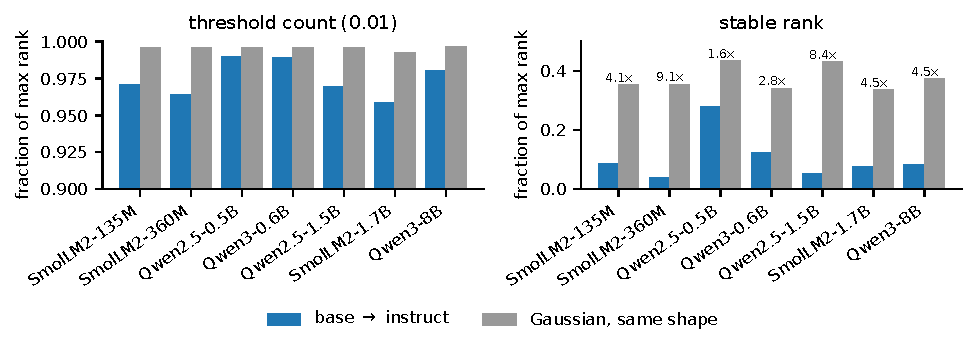
\includegraphics[width=\linewidth]{figures/released_pairs.pdf}
\end{center}
\caption{Official base $\to$ instruct updates (blue) against a Gaussian matrix of
the same shape (grey), ordered by model size. Left: the threshold count puts
every update within a few points of noise (note the axis starts at 0.9).
Right: stable rank puts every update 1.6--9.1$\times$ below noise.}
\label{fig:released}
\end{figure}

\begin{table}[t]
\caption{Released base/instruct pairs. Noise columns use a Gaussian matrix of
the same shape for every weight matrix. Last column: 95\% layer-bootstrap
interval on the ratio.}
\label{tab:released}
\begin{center}
\begin{tabular}{lccccc}
\toprule
pair & threshold & noise & stable rank & noise & noise / real \\
\midrule
SmolLM2-135M & 97.1\% & 99.6\% & 0.086 & 0.354 & 4.1 (3.5--5.0) \\
SmolLM2-360M & 96.4\% & 99.6\% & 0.039 & 0.356 & 9.1 (8.0--10.6) \\
Qwen2.5-0.5B & 99.0\% & 99.6\% & 0.280 & 0.434 & 1.6 (1.5--1.7) \\
Qwen3-0.6B   & 98.9\% & 99.6\% & 0.124 & 0.342 & 2.8 (2.6--3.0) \\
Qwen2.5-1.5B & 96.9\% & 99.6\% & 0.051 & 0.432 & 8.4 (7.7--9.2) \\
SmolLM2-1.7B & 95.9\% & 99.3\% & 0.075 & 0.336 & 4.5 (4.2--4.9) \\
Qwen3-8B     & 98.0\% & 99.6\% & 0.082 & 0.373 & 4.5 (4.2--5.0) \\
\bottomrule
\end{tabular}
\end{center}
\end{table}

Our fine-tunes are small, while released instruct models go through much
larger and mixed post-training. Figure~\ref{fig:released} and
Table~\ref{tab:released} show the same pattern on seven official pairs. The
threshold count reads 95.9--99.0\% for every update, within a few points of
noise; stable rank is 1.6--9.1$\times$ below noise for every one, including
Qwen3-8B at 4.5$\times$. The measurement problem is therefore not a property
of small runs, and it applies directly to the setting studied by prior work
on released models.

Qwen2.5-0.5B is the outlier, only 1.6$\times$ below noise and less
concentrated than our own SFT of the same base (0.280 against 0.145). We do
not know why. Nothing here says what the released post-training did, only that
its update is not noise-like.
